\documentclass[aspectratio=169]{beamer}

% -- Dark Theme Setup --
\usetheme{default}
\useoutertheme{default}
\useinnertheme{default}

% Colors
\definecolor{darkbg}{HTML}{1a1a2e}
\definecolor{darkframe}{HTML}{16213e}
\definecolor{accent}{HTML}{0f3460}
\definecolor{highlight}{HTML}{e94560}
\definecolor{codegreen}{HTML}{76b900}
\definecolor{lighttext}{HTML}{e0e0e0}
\definecolor{dimtext}{HTML}{a0a0a0}

\setbeamercolor{background canvas}{bg=darkbg}
\setbeamercolor{normal text}{fg=lighttext}
\setbeamercolor{title}{fg=white}
\setbeamercolor{frametitle}{fg=white, bg=darkframe}
\setbeamercolor{item}{fg=codegreen}
\setbeamercolor{subitem}{fg=highlight}
\setbeamercolor{itemize item}{fg=codegreen}
\setbeamercolor{itemize subitem}{fg=highlight}
\setbeamercolor{enumerate item}{fg=codegreen}
\setbeamercolor{enumerate subitem}{fg=highlight}
\setbeamercolor{block title}{fg=white, bg=accent}
\setbeamercolor{block body}{fg=lighttext, bg=darkframe}
\setbeamercolor{block title alerted}{fg=white, bg=highlight}
\setbeamercolor{block body alerted}{fg=lighttext, bg=darkframe}
\setbeamercolor{block title example}{fg=white, bg=codegreen!80!black}
\setbeamercolor{block body example}{fg=lighttext, bg=darkframe}
\setbeamercolor{structure}{fg=codegreen}
\setbeamercolor{section in toc}{fg=codegreen}
\setbeamercolor{subsection in toc}{fg=lighttext}
\setbeamercolor{caption name}{fg=codegreen}
\setbeamercolor{caption}{fg=dimtext}
\setbeamercolor{math text}{fg=white}

% Fonts
\setbeamerfont{title}{size=\Large, series=\bfseries}
\setbeamerfont{frametitle}{size=\large, series=\bfseries}

% Remove navigation symbols
\setbeamertemplate{navigation symbols}{}

% Frame title
\setbeamertemplate{frametitle}{
	\vspace{0.3cm}
	\insertframetitle
	\vspace{0.1cm}
	\textcolor{codegreen}{\rule{\textwidth}{0.4pt}}
}

% Footline with page number
\setbeamertemplate{footline}{
	\hfill\textcolor{dimtext}{\scriptsize\insertframenumber/\inserttotalframenumber}\hspace*{0.5cm}
	\vspace{3pt}
}

% Itemize markers
\setbeamertemplate{itemize item}{\textcolor{codegreen}{\raisebox{0.2ex}{\small$\blacktriangleright$}}}
\setbeamertemplate{itemize subitem}{\textcolor{highlight}{\raisebox{0.2ex}{\tiny$\blacksquare$}}}
\setbeamertemplate{caption}[numbered]

% Title page
\title{GPU Programming with CUDA and Triton}
\subtitle{From Zero to 2-Hours Hero}

\usepackage[utf8]{inputenc}
\usepackage{amsmath, amssymb, latexsym}
\usepackage{multirow}
\usepackage{multicol}
\usepackage{tikz}
\usetikzlibrary{fit, positioning}
\usepackage{dsfont}
\usepackage{caption}
\usepackage{booktabs}
\usepackage{listings}
\usepackage{hyperref}
\hypersetup{colorlinks=true, linkcolor=codegreen, urlcolor=highlight}
\input{commands.tex}

% Code listing style
\lstdefinestyle{cudastyle}{
	backgroundcolor=\color{darkframe},
	basicstyle=\ttfamily\scriptsize\color{lighttext},
	keywordstyle=\color{codegreen}\bfseries,
	stringstyle=\color{highlight},
	commentstyle=\color{dimtext}\itshape,
	numberstyle=\tiny\color{dimtext},
	numbers=left,
	numbersep=5pt,
	breaklines=true,
	frame=single,
	rulecolor=\color{accent},
	tabsize=4,
	showstringspaces=false,
}
\lstset{style=cudastyle}

\begin{document}

\frame{\titlepage}

\begin{frame}
	\frametitle{Workshop Outline}
	\tableofcontents
\end{frame}

% =============================================================================
% PART 1: WHY GPUs?
% =============================================================================
\section{Why GPU Programming?}

\begin{frame}
	\frametitle{Workshop Roadmap}
	\begin{columns}
		\begin{column}{0.5\textwidth}
			\textbf{\textcolor{codegreen}{Part 1:} Why GPUs?} \\[0.3em]
			CPU vs GPU, memory hierarchy \\[1em]
			\textbf{\textcolor{codegreen}{Part 2:} CUDA -- Vector Addition} \\[0.3em]
			Grid, blocks, threads $\rightarrow$ code \\[1em]
			\textbf{\textcolor{codegreen}{Part 3:} CUDA -- Matrix Multiply} \\[0.3em]
			Shared memory, bank conflicts, tiling
		\end{column}
		\begin{column}{0.5\textwidth}
			\textbf{\textcolor{codegreen}{Part 4:} Introduction to Triton} \\[0.3em]
			Block-level programming model \\[1em]
			\textbf{\textcolor{codegreen}{Part 5:} Triton in Practice} \\[0.3em]
			Softmax, matmul, auto-tuning \\[1em]
			\textbf{\textcolor{codegreen}{Part 6:} Wrap-Up} \\[0.3em]
			Flash Attention (bonus, if time)
		\end{column}
	\end{columns}
	\vspace{0.8em}
	\begin{block}{Hands-on exercises}
		Workshop repo: \texttt{github.com/ayghri/gpuwork} \\
		GPU playground: \texttt{leetgpu.com} -- paste code, run, view PTX \\
		Compiler explorer: \texttt{godbolt.org} -- CUDA $\rightarrow$ PTX $\rightarrow$ SASS
	\end{block}
\end{frame}

\begin{frame}
	\frametitle{CPU vs GPU: Design Philosophy}
	\begin{columns}
		\begin{column}{0.5\textwidth}
			\textbf{\textcolor{codegreen}{CPU} -- Latency-optimized}
			\begin{itemize}
				\item Few powerful cores (8--64)
				\item Large caches, branch prediction
				\item Optimized for \textit{sequential} tasks
				\item Low latency per operation
			\end{itemize}
		\end{column}
		\begin{column}{0.5\textwidth}
			\textbf{\textcolor{highlight}{GPU} -- Throughput-optimized}
			\begin{itemize}
				\item Thousands of simple cores
				\item Small caches, no branch prediction
				\item Optimized for \textit{parallel} tasks
				\item High throughput overall
			\end{itemize}
		\end{column}
	\end{columns}
	\vspace{1em}
	\begin{block}{Analogy}
		CPU = sports car (fast, one passenger) \\
		GPU = bus (slower per trip, but moves 100 people at once)
	\end{block}
\end{frame}

\begin{frame}
	\frametitle{GPU Architecture Overview}
	\begin{columns}
		\begin{column}{0.55\textwidth}
			\textbf{NVIDIA GPU hierarchy:}
			\begin{itemize}
				\item \textbf{GPU} has many \textcolor{codegreen}{Streaming Multiprocessors (SMs)}
				\item Each \textbf{SM} has:
				      \begin{itemize}
					      \item CUDA cores (INT32, FP32, FP64)
					      \item Tensor Cores (matrix ops)
					      \item Shared memory / L1 cache
					      \item Register file
					      \item Warp schedulers
				      \end{itemize}
				\item A \textbf{warp} = 32 threads executing in lockstep (SIMT)
			\end{itemize}
		\end{column}
		\begin{column}{0.45\textwidth}
			\begin{block}{Example: A100}
				\begin{itemize}
					\item 108 SMs
					\item 6912 FP32 cores
					\item 432 Tensor Cores
					\item 80 GB HBM2e
					\item 2 TB/s bandwidth
					\item 1.41 GHz boost clock
				\end{itemize}
			\end{block}
		\end{column}
	\end{columns}
\end{frame}

\begin{frame}
	\frametitle{GPU Memory Hierarchy}
	\begin{columns}
		\begin{column}{0.5\textwidth}
			\begin{center}
				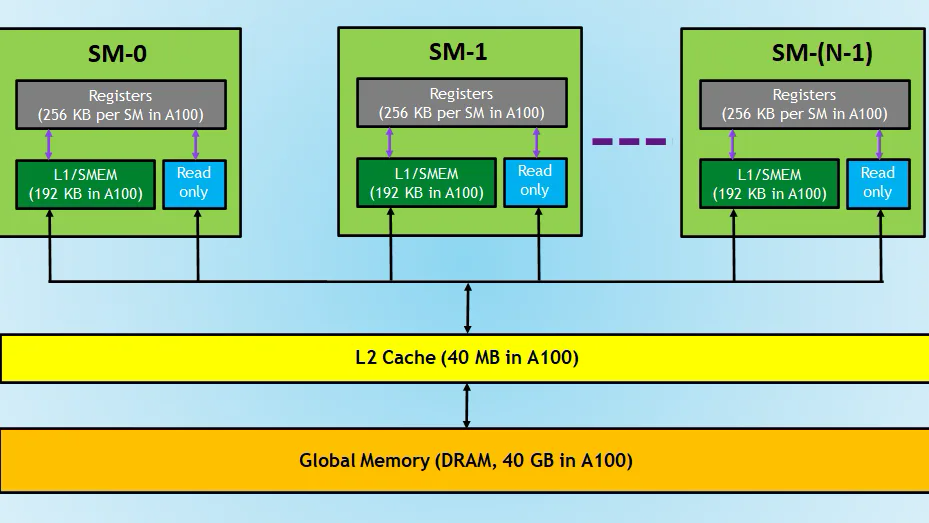
\includegraphics[width=\textwidth]{./figures/memory-hierarchy-in-gpus.png}
			\end{center}
		\end{column}
		\begin{column}{0.5\textwidth}
			\begin{center}
				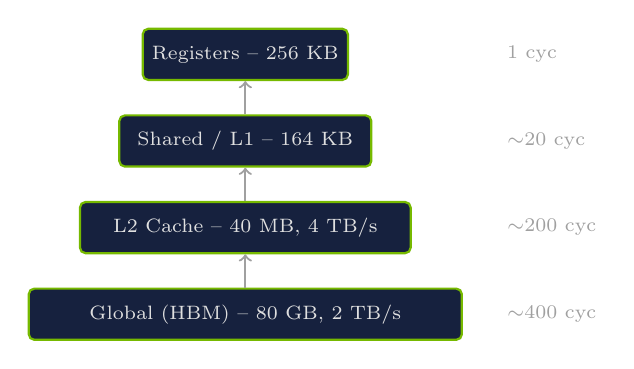
\begin{tikzpicture}[
						box/.style={draw=codegreen, fill=darkframe, text=lighttext, minimum width=2.2cm, minimum height=0.65cm, rounded corners=2pt, thick, font=\scriptsize},
						arrow/.style={->, thick, color=dimtext},
						label/.style={text=dimtext, font=\scriptsize}
					]
					\node[box, minimum width=5.5cm] (global) at (0,0) {Global (HBM) -- 80 GB, 2 TB/s};
					\node[box, minimum width=4.2cm] (l2) at (0,1.1) {L2 Cache -- 40 MB, 4 TB/s};
					\node[box, minimum width=3.2cm] (shared) at (0,2.2) {Shared / L1 -- 164 KB};
					\node[box, minimum width=2.2cm] (regs) at (0,3.3) {Registers -- 256 KB};

					\draw[arrow] (global) -- (l2);
					\draw[arrow] (l2) -- (shared);
					\draw[arrow] (shared) -- (regs);

					\node[label, right] at (3.2,0) {$\sim$400 cyc};
					\node[label, right] at (3.2,1.1) {$\sim$200 cyc};
					\node[label, right] at (3.2,2.2) {$\sim$20 cyc};
					\node[label, right] at (3.2,3.3) {1 cyc};
				\end{tikzpicture}
			\end{center}
		\end{column}
	\end{columns}
	\vspace{0.3em}
	The key to GPU performance: \textbf{keep data close to the compute}.
\end{frame}

\begin{frame}
	\frametitle{The Memory Wall}
	\begin{itemize}
		\item Most GPU kernels are \textcolor{highlight}{memory-bound}, not compute-bound
		\item A100: 312 TFLOPS (FP16) but only 2 TB/s memory bandwidth
		\item Arithmetic intensity = FLOPs / Bytes loaded
	\end{itemize}
	\vspace{0.5em}
	\begin{block}{Example: Element-wise ReLU}
		\begin{itemize}
			\item Load 1 float (4 bytes), 1 comparison, 1 store (4 bytes)
			\item Arithmetic intensity $= 1 / 8 = 0.125$ FLOP/byte
			\item Completely memory-bound -- GPU compute units are idle most of the time
		\end{itemize}
	\end{block}
	\vspace{0.5em}
	This is why \textbf{kernel fusion} matters: combine multiple operations into one kernel to reduce memory round-trips.
\end{frame}

% =============================================================================
% PART 2: CUDA — VECTOR ADDITION
% =============================================================================
\section{CUDA: Vector Addition}

\begin{frame}
	\frametitle{Grid, Blocks, and Threads}
	\begin{center}
		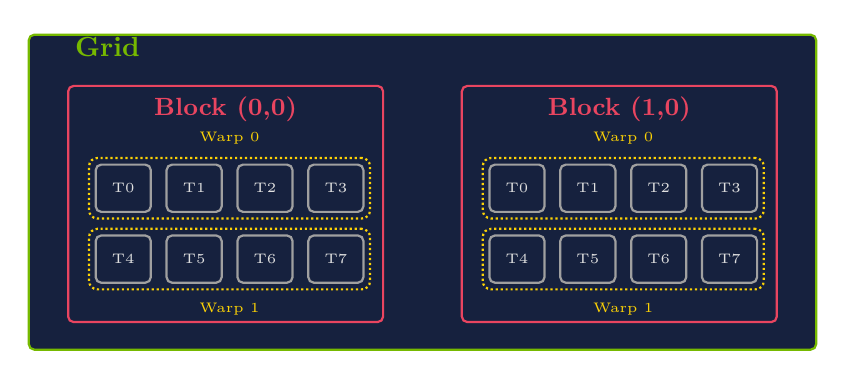
\begin{tikzpicture}[
				box/.style={draw=codegreen, fill=darkframe, text=lighttext, rounded corners=2pt, thick, minimum height=0.7cm},
				thr/.style={box, minimum width=0.7cm, minimum height=0.6cm, draw=dimtext, font=\tiny},
				warpbox/.style={draw=yellow!70!orange, densely dotted, thick, rounded corners=3pt},
				arrow/.style={->, thick, color=dimtext}
			]
			% Grid
			\node[box, minimum width=10cm, minimum height=4cm] (grid) at (0, -0.15) {};
			\node[text=codegreen, font=\bfseries] at (-4, 1.7) {Grid};

			% Block 0
			\node[box, minimum width=4cm, minimum height=3cm, draw=highlight] (b0) at (-2.5, -0.3) {};
			\node[text=highlight, font=\small\bfseries] at (-2.5, 0.9) {Block (0,0)};

			% Block 0 - Warp 0 (top row: T0-T3)
			\foreach \i in {0,...,3} {
					\node[thr] (b0t\i) at (-3.8+\i*0.9, -0.1) {T\i};
				}
			\node[warpbox, fit=(b0t0)(b0t3), inner sep=2pt] (b0w0) {};
			\node[text=yellow!70!orange, font=\tiny, above=1pt of b0w0] {Warp 0};

			% Block 0 - Warp 1 (bottom row: T4-T7)
			\foreach \i in {0,...,3} {
					\node[thr] (b0t\the\numexpr\i+4\relax) at (-3.8+\i*0.9, -1.0) {T\the\numexpr\i+4\relax};
				}
			\node[warpbox, fit=(b0t4)(b0t7), inner sep=2pt] (b0w1) {};
			\node[text=yellow!70!orange, font=\tiny, below=1pt of b0w1] {Warp 1};

			% Block 1
			\node[box, minimum width=4cm, minimum height=3cm, draw=highlight] (b1) at (2.5, -0.3) {};
			\node[text=highlight, font=\small\bfseries] at (2.5, 0.9) {Block (1,0)};

			% Block 1 - Warp 0
			\foreach \i in {0,...,3} {
					\node[thr] (b1t\i) at (1.2+\i*0.9, -0.1) {T\i};
				}
			\node[warpbox, fit=(b1t0)(b1t3), inner sep=2pt] (b1w0) {};
			\node[text=yellow!70!orange, font=\tiny, above=1pt of b1w0] {Warp 0};

			% Block 1 - Warp 1
			\foreach \i in {0,...,3} {
					\node[thr] (b1t\the\numexpr\i+4\relax) at (1.2+\i*0.9, -1.0) {T\the\numexpr\i+4\relax};
				}
			\node[warpbox, fit=(b1t4)(b1t7), inner sep=2pt] (b1w1) {};
			\node[text=yellow!70!orange, font=\tiny, below=1pt of b1w1] {Warp 1};
		\end{tikzpicture}
	\end{center}
	\vspace{0.3em}
	\begin{itemize}
		\item \textbf{Thread}: single execution unit, has a unique ID
		\item \textcolor{yellow!70!orange}{\textbf{Warp}}: group of threads executing in lockstep (32 in reality, 4 here)
		\item \textbf{\textcolor{highlight}{Block (CTA)}}: group of threads that can cooperate (shared memory, sync)
		\item \textbf{\textcolor{codegreen}{Grid}}: collection of blocks that execute a kernel
	\end{itemize}
\end{frame}

\begin{frame}
	\frametitle{Thread Indexing}
	Every thread knows \textit{who it is} via built-in variables:
	\vspace{0.5em}
	\begin{columns}
		\begin{column}{0.5\textwidth}
			\begin{block}{Built-in variables}
				\texttt{threadIdx.x, .y, .z} \\
				\quad Thread index within block \\[0.5em]
				\texttt{blockIdx.x, .y, .z} \\
				\quad Block index within grid \\[0.5em]
				\texttt{blockDim.x, .y, .z} \\
				\quad Threads per block \\[0.5em]
				\texttt{gridDim.x, .y, .z} \\
				\quad Blocks per grid
			\end{block}
		\end{column}
		\begin{column}{0.5\textwidth}
			\begin{block}{Global thread ID (1D)}
				\texttt{int i = blockIdx.x * blockDim.x} \\
				\texttt{\hspace{2.5em}  + threadIdx.x;}
				\vspace{0.5em}

				With 4 blocks of 256 threads: \\
				Block 0: threads 0--255 \\
				Block 1: threads 256--511 \\
				Block 2: threads 512--767 \\
				Block 3: threads 768--1023
			\end{block}
		\end{column}
	\end{columns}
\end{frame}

\begin{frame}[fragile]
	\frametitle{CPU Baseline: Vector Addition}
	Before writing GPU code, let's see the CPU version:
	\begin{lstlisting}[language=C, title={\color{codegreen}Sequential}]
void vec_add(const float* A, const float* B, float* C, int N) {
    for (int i = 0; i < N; i++)
        C[i] = A[i] + B[i];
}
	\end{lstlisting}
	\vspace{0.2em}
	\begin{lstlisting}[language=C, title={\color{codegreen}Parallel with OpenMP}]
void vec_add_omp(const float* A, const float* B, float* C, int N) {
    #pragma omp parallel for
    for (int i = 0; i < N; i++)
        C[i] = A[i] + B[i];
}
	\end{lstlisting}
	\vspace{0.3em}
	\begin{itemize}
		\item OpenMP parallelizes across CPU cores (8--64 threads)
		\item GPU will launch \textbf{thousands} of threads for the same work
		\item File: \texttt{00\_cpu\_vec\_add.cu}
	\end{itemize}
\end{frame}

\begin{frame}[fragile]
	\frametitle{First Kernel: Vector Addition}
	\begin{lstlisting}[language=C, title={\color{codegreen}Kernel -- runs on GPU, one instance per thread}]
__global__ void vec_add(float *a, float *b, float *c, int n) {
    int i = blockIdx.x * blockDim.x + threadIdx.x;
    if (i < n) {
        c[i] = a[i] + b[i];
    }
}
	\end{lstlisting}
	\vspace{0.5em}
	\begin{block}{Line by line}
		\begin{itemize}
			\item \texttt{\_\_global\_\_} -- marks this as a \textbf{kernel}: called from CPU, runs on GPU
			\item \texttt{blockIdx.x * blockDim.x + threadIdx.x} -- each thread computes its unique global index
			\item \texttt{if (i < n)} -- boundary guard: grid may have more threads than elements
			\item \texttt{c[i] = a[i] + b[i]} -- the actual work: each thread handles \textbf{one} element
		\end{itemize}
	\end{block}
\end{frame}

\begin{frame}[fragile]
	\frametitle{What Does the GPU Actually Run? PTX}
	\texttt{nvcc} compiles CUDA to \textbf{PTX} (Parallel Thread Execution) -- a virtual ISA for NVIDIA GPUs.
	\begin{lstlisting}[title={\color{codegreen}PTX for c[i] = a[i] + b[i] (simplified)}]
ld.global.f32  %f1, [%rd4];   // load a[i]
ld.global.f32  %f2, [%rd5];   // load b[i]
add.f32        %f3, %f1, %f2; // f3 = a[i] + b[i]
st.global.f32  [%rd6], %f3;   // store c[i]
	\end{lstlisting}
	\vspace{0.3em}
	\begin{itemize}
		\item PTX is then compiled to \textbf{SASS} (the actual machine code) for your specific GPU
		\item \texttt{nvcc -ptx vec\_add.cu} generates the PTX file
		\item LeetGPU shows the generated PTX for your submissions
		\item \texttt{godbolt.org} lets you view CUDA $\rightarrow$ PTX $\rightarrow$ SASS interactively
	\end{itemize}
	\vspace{0.3em}
	\begin{block}{Why care about PTX?}
		Reading PTX tells you what the compiler \textit{actually} did -- did it use shared memory? How many registers? Did it unroll your loop?
	\end{block}
\end{frame}

\begin{frame}[fragile]
	\frametitle{Exercise 1c: Vec Add with Inline PTX}
	\begin{block}{File: \texttt{01c\_ptx\_vec\_add.cu} {\normalfont\textcolor{dimtext}{(nvcc only -- use godbolt.org or compile locally)}}}
		You can embed PTX instructions directly in CUDA using \texttt{asm()}.
	\end{block}
	\vspace{0.3em}
	\begin{lstlisting}[language=C]
__global__ void vec_add_ptx(const float* A, const float* B,
                            float* C, int N) {
    int i = blockIdx.x * blockDim.x + threadIdx.x;
    if (i < N) {
        float a = A[i], b = B[i], c;
        asm("add.f32 %0, %1, %2;" : "=f"(c) : "f"(a), "f"(b));
        C[i] = c;
    }
}
	\end{lstlisting}
	\vspace{0.3em}
	\begin{itemize}
		\item \texttt{"add.f32 \%0, \%1, \%2"} -- the PTX instruction
		\item \texttt{"=f"(c)} -- output: float register mapped to \texttt{c}
		\item \texttt{"f"(a), "f"(b)} -- inputs: float registers mapped to \texttt{a}, \texttt{b}
	\end{itemize}
\end{frame}

\begin{frame}[fragile]
	\frametitle{Thread Identity: CUDA Built-ins and PTX Registers}
	Every thread knows who it is. Some identities are CUDA built-ins, others require PTX:
	\vspace{0.3em}
	\begin{lstlisting}[language=C, title={\color{codegreen}Works on LeetGPU}]
unsigned int laneid = threadIdx.x % 32;  // warp lane
unsigned int warpid = threadIdx.x / 32;  // warp index
	\end{lstlisting}
	\vspace{0.2em}
	\renewcommand{\arraystretch}{1.2}
	\begin{center}\scriptsize
		\begin{tabular}{l l l}
			\toprule
			\textcolor{codegreen}{CUDA built-in}                & \textcolor{codegreen}{PTX register}     & \textcolor{codegreen}{Meaning} \\
			\midrule
			\texttt{threadIdx.x/y/z}  & \texttt{\%tid.x/y/z}    & Thread index in block \\
			\texttt{blockDim.x/y/z}   & \texttt{\%ntid.x/y/z}   & Block dimensions \\
			\texttt{blockIdx.x/y/z}   & \texttt{\%ctaid.x/y/z}  & Block index in grid \\
			\texttt{gridDim.x/y/z}    & \texttt{\%nctaid.x/y/z} & Grid dimensions \\
			\texttt{threadIdx.x \% 32}& \texttt{\%laneid}        & Lane within warp (0--31) \\
			\texttt{threadIdx.x / 32} & \texttt{\%warpid}        & Warp index within block \\
			\texttt{clock()}           & \texttt{\%clock}         & Cycle counter \\
			\textit{(inline PTX only)} & \texttt{\%smid}          & Which SM runs this block \\
			\bottomrule
		\end{tabular}
	\end{center}
	\vspace{0.2em}
	\begin{itemize}
		\item File: \texttt{01d\_special\_registers.cu} -- prints warp, lane, block for each thread
	\end{itemize}
\end{frame}

\begin{frame}[fragile]
	\frametitle{Host Code: Allocate, Copy, Launch, Copy Back}
	\begin{lstlisting}[language=C]
int n = 1 << 20;  // 1M elements
size_t bytes = n * sizeof(float);

// Allocate host (CPU) and device (GPU) memory
float *h_a = (float*)malloc(bytes);     // CPU
float *d_a; cudaMalloc(&d_a, bytes);    // GPU

// Copy data: CPU -> GPU
cudaMemcpy(d_a, h_a, bytes, cudaMemcpyHostToDevice);

// Launch kernel: 4096 blocks x 256 threads = 1M threads
vec_add<<<(n+255)/256, 256>>>(d_a, d_b, d_c, n);

// Copy result: GPU -> CPU
cudaMemcpy(h_c, d_c, bytes, cudaMemcpyDeviceToHost);

// Free GPU memory
cudaFree(d_a);
	\end{lstlisting}
	\vspace{0.3em}
	\begin{center}
		\texttt{<<<grid\_size, block\_size>>>} = how many blocks, how many threads per block
	\end{center}
\end{frame}

\begin{frame}
	\frametitle{What Just Happened?}
	\begin{center}
		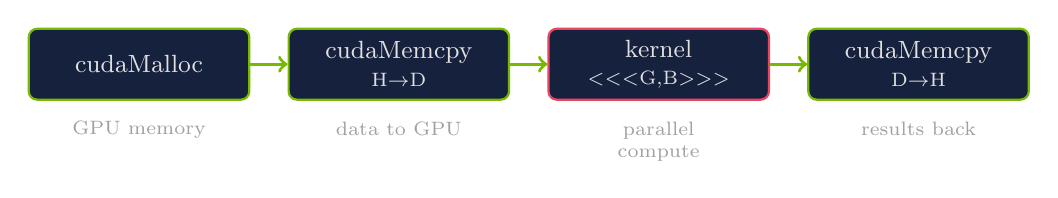
\begin{tikzpicture}[
				box/.style={draw=codegreen, fill=darkframe, text=lighttext, minimum width=2.8cm, minimum height=0.9cm, rounded corners=3pt, thick, align=center, font=\small},
				arrow/.style={->, very thick, color=codegreen},
				lbl/.style={text=dimtext, font=\scriptsize, align=center}
			]
			\node[box] (alloc) at (0, 0) {cudaMalloc};
			\node[box] (h2d) at (3.3, 0) {cudaMemcpy\\[-0.1em]\scriptsize H$\rightarrow$D};
			\node[box, draw=highlight] (kernel) at (6.6, 0) {kernel\\[-0.1em]\scriptsize$<<<$G,B$>>>$};
			\node[box] (d2h) at (9.9, 0) {cudaMemcpy\\[-0.1em]\scriptsize D$\rightarrow$H};

			\draw[arrow] (alloc) -- (h2d);
			\draw[arrow] (h2d) -- (kernel);
			\draw[arrow] (kernel) -- (d2h);

			\node[lbl, below=4pt of alloc] {GPU memory};
			\node[lbl, below=4pt of h2d] {data to GPU};
			\node[lbl, below=4pt of kernel] {parallel\\compute};
			\node[lbl, below=4pt of d2h] {results back};
		\end{tikzpicture}
	\end{center}
	\vspace{0.5em}
	\begin{itemize}
		\item CPU and GPU have \textbf{separate memory} -- data must be copied explicitly
		\item The kernel launches \textbf{asynchronously} -- CPU doesn't wait
		\item \texttt{cudaMemcpy} back to host \textbf{synchronizes} (waits for kernel to finish)
		\item For vec\_add with 1M elements: 4096 blocks $\times$ 256 threads = 1,048,576 threads launched simultaneously
	\end{itemize}
\end{frame}

\begin{frame}
	\frametitle{Warps and SIMT}
	\begin{itemize}
		\item Threads in a block are grouped into \textbf{warps} of 32 threads
		\item All threads in a warp execute the \textit{same instruction} at the same time (\textbf{SIMT})
		\item If threads in a warp diverge (different \texttt{if} branches): \\
		      $\rightarrow$ both branches execute sequentially (\textcolor{highlight}{warp divergence})
	\end{itemize}
	\vspace{0.5em}
	\begin{alertblock}{Warp Divergence -- Avoid This}
		\begin{ttfamily}\scriptsize
			if (threadIdx.x \% 2 == 0) \{ do\_A(); \} \\
			else \{ do\_B(); \}
		\end{ttfamily}
		\vspace{0.3em}

		Half the warp is idle during \texttt{do\_A()}, the other half during \texttt{do\_B()}. 50\% efficiency!
	\end{alertblock}
	\vspace{0.3em}
	In vec\_add, the \texttt{if (i < n)} guard only diverges in the \textit{last} block -- negligible cost.
\end{frame}

\begin{frame}[fragile]
	\frametitle{Exercise 1: Vector Addition}
	\begin{block}{Your turn! Open \texttt{leetgpu.com} and try it}
		File: \texttt{01\_vec\_add.cu}
	\end{block}
	\vspace{0.3em}
	\begin{lstlisting}[language=C]
__global__ void vec_add_kernel(const float* A, const float* B,
                               float* C, int N) {
    int i = 0; // TODO: compute global thread index

    // TODO: boundary check and perform addition
}
	\end{lstlisting}
	\vspace{0.3em}
	\begin{itemize}
		\item Compute \texttt{i} using \texttt{blockIdx.x}, \texttt{blockDim.x}, \texttt{threadIdx.x}
		\item Don't forget the \texttt{if (i < N)} guard!
		\item After it passes, check the PTX tab on LeetGPU -- find the \texttt{ld.global}, \texttt{add.f32}, \texttt{st.global}
	\end{itemize}
\end{frame}

\begin{frame}[fragile]
	\frametitle{Exercise 1b: Fused Vector Add + ReLU}
	\begin{block}{Try it on \texttt{leetgpu.com}}
		File: \texttt{01b\_fused\_vec\_add\_relu.cu}
	\end{block}
	\vspace{0.3em}
	Remember the \textbf{memory wall}? Two separate kernels means two HBM round-trips:
	\begin{lstlisting}[language=C]
// UNFUSED: 4 HBM accesses per element
vec_add_kernel<<<G,B>>>(A, B, tmp, N);  // read A,B -> write tmp
relu_kernel<<<G,B>>>(tmp, C, N);        // read tmp -> write C
	\end{lstlisting}
	\vspace{0.2em}
	Fuse them into \textbf{one kernel} -- only 2 HBM accesses per element:
	\begin{lstlisting}[language=C]
__global__ void fused_vec_add_relu_kernel(const float* A,
        const float* B, float* C, int N) {
    int i = blockIdx.x * blockDim.x + threadIdx.x;
    if (i < N) {
        C[i] = 0.0f; // TODO: fmaxf(A[i] + B[i], 0.0f)
    }
}
	\end{lstlisting}
	\vspace{0.2em}
	\textbf{Key takeaway}: kernel fusion = fewer memory round-trips = faster.
\end{frame}

% =============================================================================
% PART 3: CUDA — MATRIX MULTIPLY
% =============================================================================
\section{CUDA: Matrix Multiply}

\begin{frame}[fragile]
	\frametitle{Naive Matrix Multiplication}
	\begin{lstlisting}[language=C]
__global__ void matmul_naive(float *A, float *B, float *C,
                             int M, int N, int K) {
    int row = blockIdx.y * blockDim.y + threadIdx.y;
    int col = blockIdx.x * blockDim.x + threadIdx.x;

    if (row < M && col < N) {
        float sum = 0.0f;
        for (int k = 0; k < K; k++) {
            sum += A[row * K + k] * B[k * N + col];
        }
        C[row * N + col] = sum;
    }
}
	\end{lstlisting}
	\begin{itemize}
		\item Each thread computes one element of $C$ -- now using \textbf{2D} blocks/grid
		\item Launch: \texttt{dim3 block(16, 16); dim3 grid(N/16, M/16);}
		\item Problem: each element of $A$ and $B$ is loaded from \textcolor{highlight}{global memory} $K$ times!
	\end{itemize}
\end{frame}

\begin{frame}[fragile]
	\frametitle{Exercise 2: Naive Matrix Multiplication}
	\begin{block}{Try it on \texttt{leetgpu.com}}
		File: \texttt{02\_naive\_matmul.cu}
	\end{block}
	\vspace{0.3em}
	\begin{lstlisting}[language=C]
__global__ void matmul_kernel(const float* A, const float* B,
                              float* C, int M, int N, int K) {
    int row = 0; // TODO: use blockIdx.y, blockDim.y, threadIdx.y
    int col = 0; // TODO: use blockIdx.x, blockDim.x, threadIdx.x

    if (row < M && col < N) {
        float sum = 0.0f;
        // TODO: loop over K, accumulate A[row][k] * B[k][col]
        C[row * N + col] = sum;
    }
}
	\end{lstlisting}
	\vspace{0.3em}
	\begin{itemize}
		\item Row-major layout: \texttt{A[row][k]} $=$ \texttt{A[row * K + k]}
		\item Launch with \texttt{dim3 block(16, 16)} -- 256 threads per block
	\end{itemize}
\end{frame}

\begin{frame}
	\frametitle{Why the Naive Version is Slow}
	For $C = A \times B$ with $M = N = K = 4096$:
	\vspace{0.5em}
	\begin{itemize}
		\item Each thread does $K = 4096$ multiply-adds, loading 2 floats each time
		\item $16.8$M threads $\times$ $4096 \times 2 \times 4$ bytes $=$ \textbf{549 GB} of global loads
		\item But row $i$ of $A$ is needed by every element in row $i$ of $C$ (4096 times!)
		\item Same for column $j$ of $B$ -- massive redundant traffic
	\end{itemize}
	\vspace{0.5em}
	\begin{alertblock}{We need to cache and reuse data}
		Global memory: $\sim$400 cycles per access. \\
		What if we loaded a tile once into \textbf{fast on-chip memory} and reused it?
	\end{alertblock}
\end{frame}

\begin{frame}[fragile]
	\frametitle{Shared Memory: On-Chip Cache You Control}
	Fast memory shared by all threads in a block -- a programmer-managed SRAM.
	\vspace{0.3em}
	\begin{lstlisting}[language=C, title={\color{codegreen}Declaration and usage}]
__shared__ float tile[16][16]; // per-block, on-chip

// Each thread loads one element from global -> shared
tile[threadIdx.y][threadIdx.x] = A[row * K + col];
__syncthreads(); // barrier: everyone must finish loading

// Now any thread in the block can read any element -- fast
float val = tile[threadIdx.y][3]; // ~20 cycles vs ~400
	\end{lstlisting}
	\vspace{0.3em}
	\begin{itemize}
		\item \textbf{48--164 KB per SM} (configurable, shared with L1)
		\item $\sim$20 cycles latency vs $\sim$400 for global memory
		\item \texttt{\_\_syncthreads()}: barrier -- ensures all threads finished writing before any reads
	\end{itemize}
\end{frame}

\begin{frame}[fragile]
	\frametitle{Tiled Matmul: Loading Tiles into Shared Memory}
	\begin{lstlisting}[language=C]
#define TILE 16
__global__ void matmul_tiled(float *A, float *B, float *C,
                              int M, int N, int K) {
    __shared__ float As[TILE][TILE], Bs[TILE][TILE];
    int row = blockIdx.y * TILE + threadIdx.y;
    int col = blockIdx.x * TILE + threadIdx.x;
    float sum = 0.0f;

    for (int t = 0; t < (K + TILE - 1) / TILE; t++) {
        // All 256 threads collaboratively load 2 tiles
        As[threadIdx.y][threadIdx.x] =
            A[row * K + t * TILE + threadIdx.x];
        Bs[threadIdx.y][threadIdx.x] =
            B[(t * TILE + threadIdx.y) * N + col];
        __syncthreads();

        for (int k = 0; k < TILE; k++)
            sum += As[threadIdx.y][k] * Bs[k][threadIdx.x];
        __syncthreads();
    }
    C[row * N + col] = sum;
}
	\end{lstlisting}
\end{frame}

\begin{frame}
	\frametitle{Cache Reuse: Why Tiling Works}
	\begin{columns}
		\begin{column}{0.48\textwidth}
			\begin{alertblock}{Without tiling}
				Every multiply-add loads from HBM. \\[0.3em]
				Global loads: $O(MNK)$ \\
				$= 2 \times 4096^3 \times 4 \approx$ \textbf{549 GB}
			\end{alertblock}
		\end{column}
		\begin{column}{0.48\textwidth}
			\begin{exampleblock}{With tiling ($T = 16$)}
				Each tile loaded once, reused $T$ times. \\[0.3em]
				Global loads: $O(MNK / T)$ \\
				$\approx$ \textbf{34 GB} -- 16$\times$ less!
			\end{exampleblock}
		\end{column}
	\end{columns}
	\vspace{0.8em}
	\textbf{What happens inside one tile iteration:}
	\begin{enumerate}
		\item 256 threads each load 1 element of $A$ tile + 1 element of $B$ tile from global $\rightarrow$ shared
		\item \texttt{\_\_syncthreads()} -- everyone waits
		\item Each thread reads 16 elements from $A_s$ and 16 from $B_s$ --\textbf{all from shared memory}
		\item \texttt{\_\_syncthreads()} -- safe to overwrite for next tile
	\end{enumerate}
\end{frame}

\begin{frame}
	\frametitle{Shared Memory Banks}
	Shared memory is divided into \textbf{32 banks} (one per warp thread). \\
	Consecutive 4-byte words map to consecutive banks:
	\vspace{0.5em}
	\begin{center}
		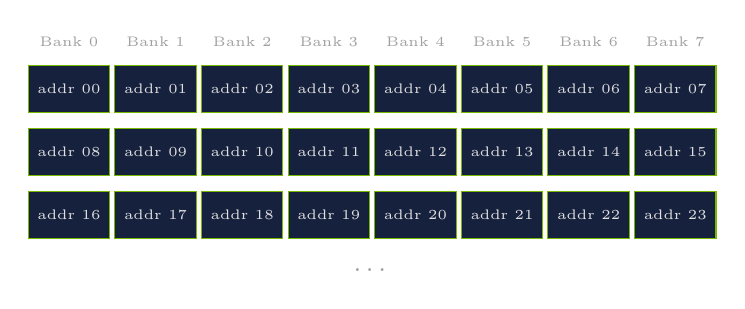
\begin{tikzpicture}[
				bank/.style={draw=codegreen, fill=darkframe, text=lighttext, minimum width=0.85cm, minimum height=0.6cm, font=\tiny},
				label/.style={text=dimtext, font=\tiny}
			]
			% Bank labels
			\foreach \i in {0,...,7} {
					\node[label] at (\i*1.1, 0.6) {Bank \i};
				}
			% Row 0
			\foreach \i in {0,...,7} {
					\node[bank] at (\i*1.1, 0) {addr 0\i};
				}
			% Row 1
			\foreach \i in {0,...,7} {
					\pgfmathtruncatemacro{\addr}{\i+8}
					\ifnum\addr<10
						\node[bank] at (\i*1.1, -0.8) {addr 0\addr};
					\else
						\node[bank] at (\i*1.1, -0.8) {addr \addr};
					\fi
				}
			% Row 2
			\foreach \i in {0,...,7} {
					\pgfmathtruncatemacro{\addr}{\i+16}
					\node[bank] at (\i*1.1, -1.6) {addr \addr};
				}
			\node[text=dimtext] at (3.85, -2.3) {\ldots};
		\end{tikzpicture}
	\end{center}
	\vspace{0.3em}
	\begin{itemize}
		\item Each bank serves one address per cycle
		\item Two threads, \textit{different addresses}, \textit{same bank}: \textcolor{highlight}{\textbf{bank conflict}} -- serialized
		\item All threads, \textit{same address}: broadcast (no conflict)
	\end{itemize}
\end{frame}

\begin{frame}
	\frametitle{Bank Conflicts in Our Matmul}
	\begin{columns}
		\begin{column}{0.48\textwidth}
			\begin{exampleblock}{\texttt{As[ty][k]} -- no conflict}
				\begin{center}
					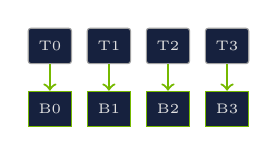
\begin{tikzpicture}[
							thr/.style={draw=dimtext, fill=darkframe, text=lighttext, minimum width=0.55cm, minimum height=0.45cm, font=\tiny, rounded corners=1pt},
							bank/.style={draw=codegreen, fill=darkframe, text=lighttext, minimum width=0.55cm, minimum height=0.45cm, font=\tiny},
							arrow/.style={->, thick, color=codegreen}
						]
						\foreach \i in {0,...,3} {
								\node[thr] (t\i) at (\i*0.75, 0.8) {T\i};
								\node[bank] (b\i) at (\i*0.75, 0) {B\i};
								\draw[arrow] (t\i) -- (b\i);
							}
					\end{tikzpicture}
				\end{center}
				All threads in a warp read the same \texttt{k}, different \texttt{ty} $\rightarrow$ different rows $\rightarrow$ different banks. \\
				\textcolor{codegreen}{No conflict}
			\end{exampleblock}
		\end{column}
		\begin{column}{0.48\textwidth}
			\begin{alertblock}{\texttt{Bs[k][tx]} -- depends on \texttt{k}}
				\begin{center}
					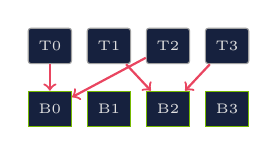
\begin{tikzpicture}[
							thr/.style={draw=dimtext, fill=darkframe, text=lighttext, minimum width=0.55cm, minimum height=0.45cm, font=\tiny, rounded corners=1pt},
							bank/.style={draw=codegreen, fill=darkframe, text=lighttext, minimum width=0.55cm, minimum height=0.45cm, font=\tiny},
							arrow/.style={->, thick, color=highlight}
						]
						\foreach \i in {0,...,3} {
								\node[thr] (t\i) at (\i*0.75, 0.8) {T\i};
							}
						\foreach \i in {0,...,3} {
								\node[bank] (b\i) at (\i*0.75, 0) {B\i};
							}
						\draw[arrow] (t0) -- (b0);
						\draw[arrow] (t1) -- (b2);
						\draw[arrow] (t2) -- (b0);
						\draw[arrow] (t3) -- (b2);
					\end{tikzpicture}
				\end{center}
				If row stride is a multiple of 32, threads reading different columns can hit the same bank. \\
				\textcolor{highlight}{Potential conflict!}
			\end{alertblock}
		\end{column}
	\end{columns}
\end{frame}

\begin{frame}
	\frametitle{Fixing Bank Conflicts: Padding}
	\begin{block}{The trick: add one extra column}
		\texttt{\scriptsize \_\_shared\_\_ float Bs[TILE][TILE];} \hfill \textcolor{highlight}{$\leftarrow$ stride 16: bank conflicts on column access} \\[0.3em]
		\texttt{\scriptsize \_\_shared\_\_ float Bs[TILE][TILE + 1];} \hfill \textcolor{codegreen}{$\leftarrow$ stride 17: no conflicts}
		\vspace{0.3em}

		The padding shifts each row by one bank, breaking the conflict pattern. \\
		Cost: 16 extra floats (64 bytes) of shared memory per tile -- negligible.
	\end{block}
	\vspace{0.5em}
	\begin{block}{Other strategies}
		\begin{itemize}
			\item Rearrange access patterns so threads hit consecutive banks
			\item Use warp-level shuffles (\texttt{\_\_shfl\_sync}) to exchange data without shared memory
			\item Profile with \texttt{ncu} -- it reports bank conflicts directly
		\end{itemize}
	\end{block}
\end{frame}

\begin{frame}[fragile]
	\frametitle{Exercise 3: Tiled Matmul with Shared Memory}
	\begin{block}{Try it on \texttt{leetgpu.com}}
		File: \texttt{03\_tiled\_matmul.cu}
	\end{block}
	\vspace{0.3em}
	\begin{lstlisting}[language=C]
// Inside the tile loop:

// TODO: load one element each into shared memory
As[threadIdx.y][threadIdx.x] = A[???];
Bs[threadIdx.y][threadIdx.x] = B[???];
__syncthreads();

// TODO: accumulate from shared memory
for (int k = 0; k < TILE; k++)
    sum += As[???][???] * Bs[???][???];
__syncthreads();
	\end{lstlisting}
	\vspace{0.3em}
	\begin{itemize}
		\item Tile $t$ starts at column \texttt{t*TILE} for $A$, row \texttt{t*TILE} for $B$
		\item Add boundary checks (load \texttt{0.0f} if out of bounds)
		\item Compare performance with your Exercise 2 solution!
		\item Check the PTX: look for \texttt{ld.shared} instead of \texttt{ld.global} in the inner loop
	\end{itemize}
\end{frame}

\begin{frame}[fragile]
	\frametitle{Exercise 4: Fix Bank Conflicts}
	\begin{block}{Try it on \texttt{leetgpu.com}}
		File: \texttt{04\_bank\_conflict\_fix.cu}
	\end{block}
	\vspace{0.5em}
	Take your working tiled matmul from Exercise 3 and:
	\begin{enumerate}
		\item Run it as-is and note the performance
		\item Change the \texttt{Bs} declaration from:
		      \begin{lstlisting}[language=C]
__shared__ float Bs[TILE][TILE];       // bank conflicts
		      \end{lstlisting}
		      to:
		      \begin{lstlisting}[language=C]
__shared__ float Bs[TILE][TILE + 1];   // no conflicts
		      \end{lstlisting}
		\item Run again -- do you see a speedup?
	\end{enumerate}
	\vspace{0.3em}
	\begin{exampleblock}{What to expect}
		The improvement depends on matrix size and GPU. \\
		On large matrices, padding can give 5--15\% speedup.
	\end{exampleblock}
\end{frame}

\begin{frame}
	\frametitle{CUDA Optimization Summary}
	\begin{enumerate}
		\item \textbf{Coalesce global memory}: consecutive threads $\rightarrow$ consecutive addresses
		\item \textbf{Cache in shared memory}: load tiles, reuse across threads
		\item \textbf{Avoid bank conflicts}: pad shared memory arrays
		\item \textbf{Minimize warp divergence}: avoid branching within warps
		\item \textbf{Maximize occupancy}: enough blocks/threads to keep SMs busy
	\end{enumerate}
	\vspace{0.5em}
	\begin{block}{Profiling tools}
		\texttt{nsys} (Nsight Systems) -- timeline view \\
		\texttt{ncu} (Nsight Compute) -- kernel-level metrics (bank conflicts, occupancy, \ldots)
	\end{block}
\end{frame}

\begin{frame}
	\frametitle{What About Tensor Cores?}
	Our tiled matmul uses \textbf{FP32 CUDA cores} -- one multiply-add per core per cycle. \\
	Modern GPUs have \textbf{Tensor Cores}: dedicated matrix-multiply units.
	\vspace{0.5em}
	\begin{block}{Tensor Core MMA (Matrix Multiply-Accumulate)}
		\begin{itemize}
			\item Computes a small matrix multiply (e.g.\ $16 \times 16 \times 16$) in \textbf{one operation}
			\item A100: \textbf{312 TFLOPS} (FP16) vs 19.5 TFLOPS (FP32 CUDA cores) -- 16$\times$ faster
			\item Requires specific data layouts in registers across threads in a warp
		\end{itemize}
	\end{block}
	\vspace{0.5em}
	\begin{alertblock}{The catch: thread-level data layout}
		Each of the 32 warp threads holds a \textit{fragment} of the tile in its registers. \\
		The layout depends on the GPU architecture (Volta, Ampere, Hopper\ldots). \\
		Getting this right in CUDA requires \texttt{wmma} or \texttt{mma.sync} PTX intrinsics -- complex!
	\end{alertblock}
\end{frame}

\begin{frame}
	\frametitle{From CUDA Pain to Triton}
	Writing high-performance CUDA is hard:
	\begin{itemize}
		\item Manual memory management, tiling, synchronization
		\item Bank conflict avoidance, memory coalescing
		\item Tensor Core usage requires warp-level register fragment layouts
		\item Different optimizations per GPU architecture
		\item Hundreds of lines for a ``simple'' matmul
	\end{itemize}
	\vspace{0.5em}
	\begin{center}
		\textcolor{codegreen}{\large What if the compiler handled all of that?}
	\end{center}
	\vspace{0.5em}
	\begin{block}{Triton's promise}
		You write block-level Python. The compiler generates: \\
		shared memory staging, bank-conflict-free layouts, coalesced loads, \\
		and \textbf{Tensor Core instructions} -- automatically.
	\end{block}
\end{frame}

% =============================================================================
% PART 4: INTRODUCTION TO TRITON
% =============================================================================
\section{Introduction to Triton}

\begin{frame}
	\frametitle{What is Triton?}
	\begin{itemize}
		\item Open-source language and compiler by OpenAI (2021)
		\item Write GPU kernels in \textbf{Python} with near-CUDA performance
		\item Key idea: program at the \textbf{block level}, not the thread level
		\item The compiler handles:
		      \begin{itemize}
			      \item Shared memory management
			      \item Memory coalescing
			      \item Warp-level optimizations
			      \item Tensor Core utilization
		      \end{itemize}
	\end{itemize}
	\vspace{0.5em}
	\begin{block}{Why Triton?}
		\begin{itemize}
			\item $\sim$10$\times$ less code than equivalent CUDA
			\item 90--100\% of hand-tuned CUDA performance
			\item Python-native: integrates with PyTorch seamlessly
			\item Active development, used in production (PyTorch 2.0 \texttt{torch.compile})
		\end{itemize}
	\end{block}
\end{frame}

\begin{frame}
	\frametitle{CUDA vs Triton: Programming Model}
	\begin{columns}
		\begin{column}{0.5\textwidth}
			\textbf{\textcolor{highlight}{CUDA}: Thread-level}
			\begin{itemize}
				\item You write code for \textit{one thread}
				\item You manage:
				      \begin{itemize}
					      \item Thread indexing
					      \item Shared memory
					      \item Synchronization
					      \item Memory coalescing
				      \end{itemize}
				\item Full control, full responsibility
			\end{itemize}
		\end{column}
		\begin{column}{0.5\textwidth}
			\textbf{\textcolor{codegreen}{Triton}: Block-level}
			\begin{itemize}
				\item You write code for \textit{one block}
				\item Compiler manages:
				      \begin{itemize}
					      \item Thread mapping
					      \item Shared memory
					      \item Synchronization
					      \item Memory coalescing
				      \end{itemize}
				\item Less control, less boilerplate
			\end{itemize}
		\end{column}
	\end{columns}
	\vspace{1em}
	\begin{center}
		In Triton, you think in \textbf{tiles/blocks of data}, not individual elements.
	\end{center}
\end{frame}

\begin{frame}
	\frametitle{Triton Core Concepts}
	\begin{itemize}
		\item \textbf{Program}: a Triton kernel -- one instance per block
		\item \texttt{tl.program\_id(axis)}: like \texttt{blockIdx} in CUDA
		\item \texttt{tl.arange(0, N)}: creates a vector \texttt{[0, 1, ..., N-1]} within a block
		\item \texttt{tl.load(ptr)}: loads a block of data from global memory
		\item \texttt{tl.store(ptr, val)}: stores a block of data to global memory
		\item \textbf{Masking}: \texttt{tl.load(ptr, mask=mask, other=0.0)} for boundary handling
	\end{itemize}
	\vspace{0.5em}
	\begin{block}{Key difference from NumPy/PyTorch}
		Operations in Triton are \textbf{block-local}: each kernel instance operates on its own tile.
		There is no implicit broadcasting across the entire tensor.
	\end{block}
\end{frame}

% =============================================================================
% PART 5: TRITON IN PRACTICE
% =============================================================================
\section{Triton in Practice}

\begin{frame}[fragile]
	\frametitle{Triton: Vector Addition}
	\begin{lstlisting}[language=Python]
import triton
import triton.language as tl

@triton.jit
def vec_add_kernel(a_ptr, b_ptr, c_ptr, n,
                   BLOCK: tl.constexpr):
    pid = tl.program_id(0)
    offsets = pid * BLOCK + tl.arange(0, BLOCK)
    mask = offsets < n

    a = tl.load(a_ptr + offsets, mask=mask)
    b = tl.load(b_ptr + offsets, mask=mask)
    tl.store(c_ptr + offsets, a + b, mask=mask)
	\end{lstlisting}
	\vspace{0.3em}
	\begin{lstlisting}[language=Python, title={\color{codegreen}Launching the kernel}]
grid = lambda meta: (triton.cdiv(n, meta['BLOCK']),)
vec_add_kernel[grid](a, b, c, n, BLOCK=1024)
	\end{lstlisting}
	\vspace{0.3em}
	Compare: 6 lines of kernel code vs 25+ lines in CUDA (with host code).
\end{frame}

\begin{frame}
	\frametitle{Exercise 5: Triton Vector Addition}
	\begin{block}{Run locally (requires GPU + \texttt{pip install triton torch})}
		File: \texttt{05\_triton\_vec\_add.py}
	\end{block}
	\vspace{0.5em}
	\begin{itemize}
		\item The file is a complete, working Triton vec\_add -- run it and read through the code
		\item Compare with your CUDA Exercise 1:
		      \begin{itemize}
			      \item No \texttt{cudaMalloc}, no \texttt{cudaMemcpy} -- PyTorch handles memory
			      \item \texttt{tl.program\_id(0)} $\equiv$ \texttt{blockIdx.x}
			      \item \texttt{tl.arange(0, BLOCK)} creates a vector of indices -- no manual thread indexing
			      \item \texttt{mask = offsets < N} replaces the \texttt{if (i < N)} guard
		      \end{itemize}
		\item Try changing \texttt{BLOCK=1024} to other values -- how does it affect performance?
	\end{itemize}
\end{frame}

\begin{frame}[fragile]
	\frametitle{Triton: Fused Softmax}
	Computing $\text{softmax}(x)_i = e^{x_i - \max(x)} / \sum_j e^{x_j - \max(x)}$ \\[0.5em]
	In PyTorch: 5 global memory round-trips (max, subtract, exp, sum, divide). \\
	In Triton: \textbf{one kernel}, data stays in SRAM.
	\begin{lstlisting}[language=Python]
@triton.jit
def softmax_kernel(input_ptr, output_ptr, n_cols,
                   BLOCK: tl.constexpr):
    row = tl.program_id(0)
    offsets = tl.arange(0, BLOCK)
    mask = offsets < n_cols

    # Load one row
    row_ptr = input_ptr + row * n_cols
    x = tl.load(row_ptr + offsets, mask=mask,
                other=-float('inf'))
    # Compute softmax in SRAM
    x_max = tl.max(x, axis=0)
    numerator = tl.exp(x - x_max)
    denominator = tl.sum(numerator, axis=0)
    result = numerator / denominator

    out_ptr = output_ptr + row * n_cols
    tl.store(out_ptr + offsets, result, mask=mask)
	\end{lstlisting}
\end{frame}

\begin{frame}
	\frametitle{Why Fused Softmax is Faster}
	\begin{columns}
		\begin{column}{0.48\textwidth}
			\textbf{\textcolor{highlight}{PyTorch (unfused)}}
			\begin{enumerate}
				\item Read $X$, write $\max(X)$
				\item Read $X, \max(X)$, write $X - \max$
				\item Read $X{-}\max$, write $\exp(X{-}\max)$
				\item Read $\exp$, write $\sum \exp$
				\item Read $\exp, \sum$, write result
			\end{enumerate}
			\textcolor{highlight}{5 kernel launches}, 5 global memory round-trips
		\end{column}
		\begin{column}{0.48\textwidth}
			\textbf{\textcolor{codegreen}{Triton (fused)}}
			\begin{enumerate}
				\item Read $X$ into SRAM
				\item Compute everything in SRAM
				\item Write result
			\end{enumerate}
			\vspace{2.1em}
			\textcolor{codegreen}{1 kernel launch}, 1 read + 1 write
		\end{column}
	\end{columns}
	\vspace{1em}
	Typical speedup: \textbf{2--4$\times$} over PyTorch for memory-bound ops.
\end{frame}

\begin{frame}
	\frametitle{Exercise 6: Triton Fused Softmax}
	\begin{block}{Run locally}
		File: \texttt{06\_triton\_softmax.py}
	\end{block}
	\vspace{0.5em}
	\begin{itemize}
		\item Run the file -- it computes row-wise softmax and checks against \texttt{torch.softmax}
		\item Read the kernel: one \texttt{tl.load}, all compute in SRAM, one \texttt{tl.store}
		\item Try these experiments:
		      \begin{itemize}
			      \item Change the matrix to \texttt{(128, 8192)} -- does it still work? (hint: \texttt{BLOCK} must be $\geq$ \texttt{n\_cols})
			      \item What happens if you remove \texttt{other=-float("inf")} from the load?
			      \item Time it vs \texttt{torch.softmax} using \texttt{torch.cuda.Event} for large matrices
		      \end{itemize}
	\end{itemize}
\end{frame}

\begin{frame}[fragile]
	\frametitle{Triton: Matrix Multiplication (1/2)}
	\begin{lstlisting}[language=Python]
@triton.jit
def matmul_kernel(
    A, B, C, M, N, K,
    stride_am, stride_ak, stride_bk, stride_bn,
    stride_cm, stride_cn,
    BLOCK_M: tl.constexpr, BLOCK_N: tl.constexpr,
    BLOCK_K: tl.constexpr,
):
    pid_m = tl.program_id(0)
    pid_n = tl.program_id(1)
    # Block starting row/col
    rm = pid_m * BLOCK_M + tl.arange(0, BLOCK_M)
    rn = pid_n * BLOCK_N + tl.arange(0, BLOCK_N)
    rk = tl.arange(0, BLOCK_K)

    # Pointers to first tiles of A and B
    A_ptrs = A + rm[:, None] * stride_am + rk[None, :] * stride_ak
    B_ptrs = B + rk[:, None] * stride_bk + rn[None, :] * stride_bn
    acc = tl.zeros((BLOCK_M, BLOCK_N), dtype=tl.float32)
	\end{lstlisting}
\end{frame}

\begin{frame}[fragile]
	\frametitle{Triton: Matrix Multiplication (2/2)}
	\begin{lstlisting}[language=Python]
    # Tiled loop over K dimension
    for k in range(0, K, BLOCK_K):
        a = tl.load(A_ptrs, mask=
            (rm[:, None] < M) & (rk[None, :] + k < K),
            other=0.0)
        b = tl.load(B_ptrs, mask=
            (rk[:, None] + k < K) & (rn[None, :] < N),
            other=0.0)
        acc += tl.dot(a, b)
        A_ptrs += BLOCK_K * stride_ak
        B_ptrs += BLOCK_K * stride_bk

    # Store result
    C_ptrs = C + rm[:, None] * stride_cm + rn[None, :] * stride_cn
    mask = (rm[:, None] < M) & (rn[None, :] < N)
    tl.store(C_ptrs, acc, mask=mask)
	\end{lstlisting}
	\vspace{0.3em}
	\begin{itemize}
		\item \texttt{tl.dot}: compiles to Tensor Core instructions (when available)
		\item Shared memory, tiling, coalescing: all handled by the compiler
		\item $\sim$30 lines vs $\sim$150+ lines for an optimized CUDA matmul
	\end{itemize}
\end{frame}

\begin{frame}[fragile]
	\frametitle{Auto-Tuning in Triton}
	Triton can automatically search for the best kernel configuration:
	\begin{lstlisting}[language=Python]
@triton.autotune(
    configs=[
        triton.Config({'BLOCK_M': 128, 'BLOCK_N': 128,
                       'BLOCK_K': 32}, num_warps=8),
        triton.Config({'BLOCK_M': 64, 'BLOCK_N': 256,
                       'BLOCK_K': 32}, num_warps=8),
        triton.Config({'BLOCK_M': 256, 'BLOCK_N': 64,
                       'BLOCK_K': 32}, num_warps=4),
        triton.Config({'BLOCK_M': 128, 'BLOCK_N': 64,
                       'BLOCK_K': 64}, num_warps=4),
    ],
    key=['M', 'N', 'K'],  # re-tune when shapes change
)
@triton.jit
def matmul_kernel(A, B, C, M, N, K, ...):
    ...
	\end{lstlisting}
	\vspace{0.3em}
	Triton benchmarks all configs on first call, caches the winner.
\end{frame}

\begin{frame}
	\frametitle{Exercise 7: Triton Matrix Multiplication}
	\begin{block}{Run locally}
		File: \texttt{07\_triton\_matmul.py}
	\end{block}
	\vspace{0.5em}
	\begin{itemize}
		\item Run the file -- it multiplies two 512$\times$512 matrices and checks against \texttt{torch.mm}
		\item Compare the code with your CUDA tiled matmul (Exercise 3):
		      \begin{itemize}
			      \item No \texttt{\_\_shared\_\_}, no \texttt{\_\_syncthreads()} -- compiler handles it
			      \item \texttt{tl.dot(a, b)} compiles to Tensor Core instructions automatically
			      \item Boundary masking via \texttt{mask=} instead of manual \texttt{if} checks
		      \end{itemize}
		\item Try experiments:
		      \begin{itemize}
			      \item Increase to 2048$\times$2048 -- how does Triton compare to \texttt{torch.mm} (cuBLAS)?
			      \item Change \texttt{BLOCK\_M/N/K} values -- what gives best performance?
		      \end{itemize}
	\end{itemize}
\end{frame}

% =============================================================================
% WRAP-UP
% =============================================================================
\section{Wrap-Up}

\begin{frame}
	\frametitle{CUDA vs Triton: When to Use What?}
	\renewcommand{\arraystretch}{1.3}
	\begin{center}
		\begin{tabular}{l c c}
			\toprule
			                          & \textcolor{highlight}{CUDA}  & \textcolor{codegreen}{Triton} \\
			\midrule
			Learning curve            & Steep                        & Gentle                        \\
			Code length               & Verbose                      & Concise                       \\
			Peak performance          & Highest                      & Near-CUDA                     \\
			Thread-level control      & Full                         & Limited                       \\
			Shared memory control     & Manual                       & Automatic                     \\
			Auto-tuning               & Manual/external              & Built-in                      \\
			Warp-level primitives     & Yes                          & Limited                       \\
			Non-NVIDIA GPUs           & No                           & Experimental (AMD)            \\
			PyTorch integration       & Requires C++ bindings        & Native                        \\
			Best for                  & Libraries, max perf          & Custom ops, research          \\
			\bottomrule
		\end{tabular}
	\end{center}
\end{frame}

\begin{frame}[fragile]
	\frametitle{The GPU Programming Landscape}
	\begin{center}
		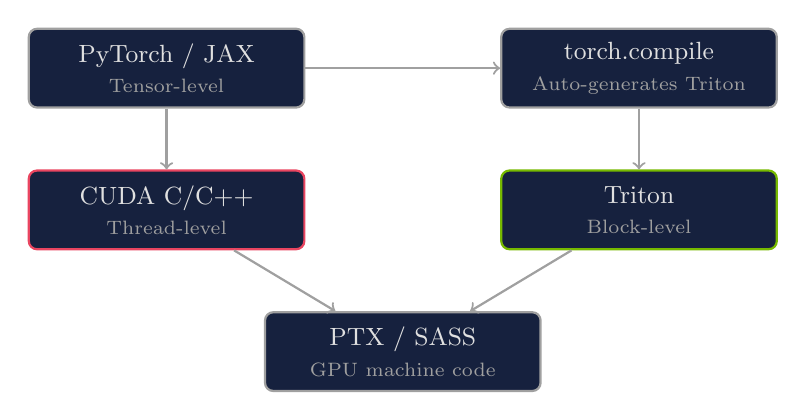
\begin{tikzpicture}[
				box/.style={draw=#1, fill=darkframe, text=lighttext, minimum width=3.5cm, minimum height=1cm, rounded corners=3pt, thick, align=center, font=\small},
				arrow/.style={->, thick, color=dimtext}
			]
			% Bottom layer
			\node[box=dimtext] (ptx) at (0, 0) {PTX / SASS \\ \scriptsize\textcolor{dimtext}{GPU machine code}};

			% Middle layer
			\node[box=highlight] (cuda) at (-3, 1.8) {CUDA C/C++ \\ \scriptsize\textcolor{dimtext}{Thread-level}};
			\node[box=codegreen] (triton) at (3, 1.8) {Triton \\ \scriptsize\textcolor{dimtext}{Block-level}};

			% Top layer
			\node[box=dimtext] (torch) at (-3, 3.6) {PyTorch / JAX \\ \scriptsize\textcolor{dimtext}{Tensor-level}};
			\node[box=dimtext] (compile) at (3, 3.6) {torch.compile \\ \scriptsize\textcolor{dimtext}{Auto-generates Triton}};

			\draw[arrow] (torch) -- (cuda);
			\draw[arrow] (torch) -- (compile);
			\draw[arrow] (compile) -- (triton);
			\draw[arrow] (cuda) -- (ptx);
			\draw[arrow] (triton) -- (ptx);
		\end{tikzpicture}
	\end{center}
	\vspace{0.3em}
	\texttt{torch.compile} (PyTorch 2.0+) auto-generates Triton kernels from eager PyTorch code -- often good enough!
\end{frame}

\begin{frame}
	\frametitle{Summary}
	\begin{enumerate}
		\item \textbf{GPUs} are throughput machines -- thousands of cores, memory hierarchy is key
		\item \textbf{CUDA} gives full control: grid $\rightarrow$ blocks $\rightarrow$ warps $\rightarrow$ threads
		      \begin{itemize}
			      \item Shared memory for cache reuse, but you manage tiling, sync, bank conflicts
			      \item Tensor Cores are fast but require complex warp-level layouts
		      \end{itemize}
		\item \textbf{Triton} raises the abstraction: block-level programming in Python
		      \begin{itemize}
			      \item Compiler handles shared memory, coalescing, Tensor Cores
			      \item Built-in auto-tuning, native PyTorch integration
		      \end{itemize}
		\item \textbf{Kernel fusion} is the single biggest optimization for most workloads
	\end{enumerate}
	\vspace{0.5em}
	\begin{block}{Resources}
		Workshop files: \texttt{github.com/ayghri/gpuwork} \\
		Triton: \texttt{triton-lang.org} ~|~
		CUDA: \texttt{docs.nvidia.com/cuda} \\
		PTX ISA: \texttt{docs.nvidia.com/cuda/parallel-thread-execution} \\
		Compiler Explorer: \texttt{godbolt.org} ~|~
		GPU MODE: YouTube / Discord
	\end{block}
	\vspace{0.5em}
	\begin{center}
		\Large\textcolor{codegreen}{Questions?}
	\end{center}
\end{frame}

% =============================================================================
% BONUS: IF TIME ALLOWS
% =============================================================================
\section{Bonus: Flash Attention}

\begin{frame}
	\begin{center}
		\vspace{2em}
		{\Large\textcolor{codegreen}{Bonus Material}} \\[1em]
		{\large If time allows: Flash Attention}
	\end{center}
\end{frame}

\begin{frame}
	\frametitle{Flash Attention: The Idea}
	Standard attention: $\text{Attention}(Q, K, V) = \text{softmax}\!\left(\frac{QK^\top}{\sqrt{d}}\right)V$
	\vspace{0.5em}
	\begin{columns}
		\begin{column}{0.48\textwidth}
			\textbf{\textcolor{highlight}{Standard implementation}}
			\begin{enumerate}
				\item Compute $S = QK^\top$ -- $O(n^2 d)$
				\item Store full $n \times n$ matrix $S$
				\item Compute $\text{softmax}(S)$ row-wise
				\item Compute $\text{softmax}(S) \cdot V$
			\end{enumerate}
			Memory: $O(n^2)$ -- explodes for long sequences
		\end{column}
		\begin{column}{0.48\textwidth}
			\textbf{\textcolor{codegreen}{Flash Attention}}
			\begin{enumerate}
				\item Tile $Q, K, V$ into blocks
				\item For each block of $Q$: iterate over $K, V$ blocks
				\item Compute local softmax with online correction
				\item Never materialize full $n \times n$ matrix
			\end{enumerate}
			Memory: $O(n)$ -- fits in SRAM!
		\end{column}
	\end{columns}
	\vspace{0.5em}
	\textbf{Result}: 2--4$\times$ faster, uses $\sim$$10{-}20\times$ less memory.
\end{frame}

\begin{frame}
	\frametitle{Online Softmax: The Key Trick}
	How to compute softmax without seeing all values at once?
	\vspace{0.5em}

	Process blocks $B_1, B_2, \ldots$ incrementally:
	\begin{enumerate}
		\item After block $B_1$: compute $m_1 = \max(B_1)$, $\ell_1 = \sum e^{B_1 - m_1}$
		\item After block $B_2$: update running max $m_2 = \max(m_1, \max(B_2))$
		\item \textbf{Rescale} previous result: $\ell_1' = \ell_1 \cdot e^{m_1 - m_2}$
		\item Accumulate: $\ell_2 = \ell_1' + \sum e^{B_2 - m_2}$
	\end{enumerate}
	\vspace{0.5em}
	\begin{block}{Applied to attention}
		\begin{itemize}
			\item Maintain running output $O$, running max $m$, running sum $\ell$
			\item For each new $K, V$ block: rescale $O$ by the max correction factor
			\item Mathematically exact -- not an approximation!
		\end{itemize}
	\end{block}
\end{frame}

\begin{frame}[fragile]
	\frametitle{Flash Attention in Triton (Sketch)}
	\begin{lstlisting}[language=Python]
@triton.jit
def flash_attn_kernel(Q, K, V, Out, ...):
    # This program handles one block of Q rows
    q_block = tl.load(Q_block_ptr)  # [BLOCK_M, d]
    m_i = tl.full([BLOCK_M], -float('inf'), tl.float32)
    l_i = tl.zeros([BLOCK_M], dtype=tl.float32)
    acc = tl.zeros([BLOCK_M, D], dtype=tl.float32)

    for j in range(0, N, BLOCK_N):  # iterate K/V blocks
        k_block = tl.load(K_block_ptr)  # [BLOCK_N, d]
        v_block = tl.load(V_block_ptr)  # [BLOCK_N, d]
        # Compute QK^T for this block
        s = tl.dot(q_block, tl.trans(k_block)) / sqrt_d
        # Online softmax update
        m_new = tl.maximum(m_i, tl.max(s, axis=1))
        alpha = tl.exp(m_i - m_new)
        p = tl.exp(s - m_new[:, None])
        l_i = l_i * alpha + tl.sum(p, axis=1)
        acc = acc * alpha[:, None] + tl.dot(p, v_block)
        m_i = m_new
    tl.store(Out_ptr, acc / l_i[:, None])
	\end{lstlisting}
\end{frame}

\end{document}
